\documentclass[bigchapter,type=bsc,colorback,accentcolor=tud11d]{tudthesis}

%\usepackage{ngerman}   ...ist ja gar nicht auf deutsch!
\usepackage{booktabs}
\usepackage{tabularx}
\usepackage{todonotes}

\usepackage{varwidth}

\usepackage{graphicx}
\usepackage{wrapfig}

% new page for each section
%\usepackage{titlesec}
%\newcommand{\sectionbreak}{\clearpage}

% flow charts etc.
\usepackage{tikz}
\usetikzlibrary{shapes,arrows,positioning,automata}

% increase line height
\renewcommand{\baselinestretch}{1.2} 


% german month for TUDthesis
\newcommand{\getmydate}{%
	\ifcase\month%
	\or Januar\or Februar\or M\"arz%
	\or April\or Mai\or Juni\or Juli%
	\or August\or September\or Oktober%
	\or November\or Dezember%
	\fi\ \number\year%
}

%--------------------------------------------------------------------------------

\begin{document}


%=====================================================================
% Title Page
%=====================================================================

\thesistitle{Optimierte Zusammenarbeit von HTTP/2 und Multipath-TCP-Schedulern}{Optimizing Cooperation of HTTP/2 and the Multipath TCP Scheduler}
\author{Maxi Weller}
\referee{Prof. Ralf Steinmetz}{Alexander Fr�mmgen}
\department{Fachbereich Informatik}
\group{Multimedia Communications Lab }
\tuprints{57580}{5758}
\makethesistitle
\affidavit{M. Weller}


%=====================================================================
\begin{abstract}
%=====================================================================

this is the content of the abstract environment
\end{abstract}




%=====================================================================
\renewcommand{\contentsname}{Contents}
%=====================================================================

\tableofcontents




%=====================================================================
\chapter{Introduction}
%=====================================================================


In the following paragraphs, we describe the motivation for the relatively recent protocols this work is based on as well as for the kind of optimizations that will be implemented in this thesis. We introduce the approach and give an overview of the remaining chapters.


%=== Motivation ========
\paragraph{Motivation}

\begin{wrapfigure}{r}{0.45\textwidth}
	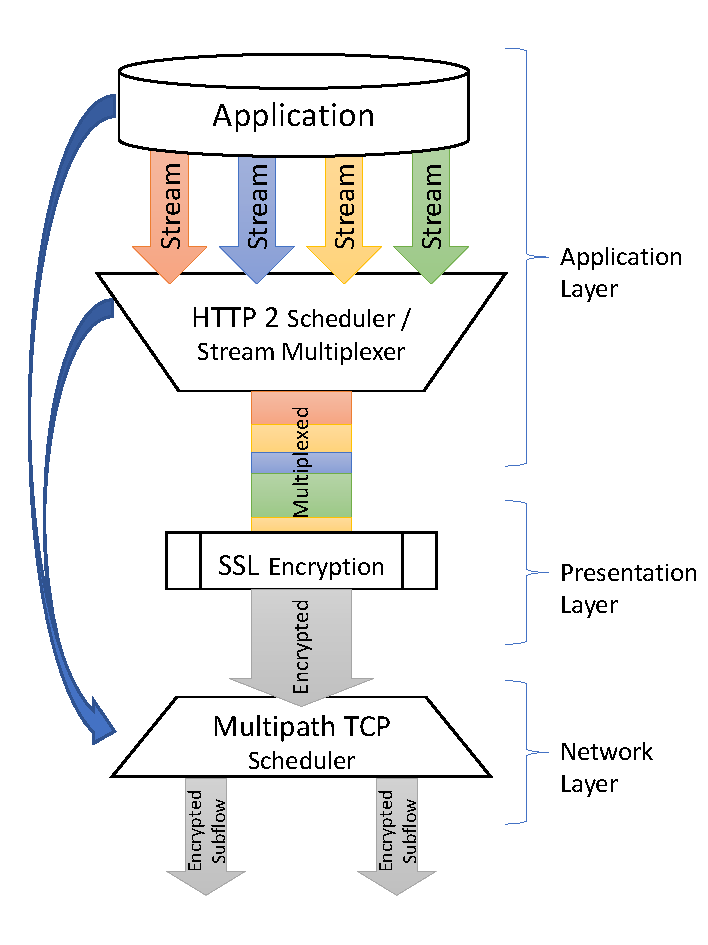
\includegraphics[width=0.4\textwidth]{mux-demux.pdf}
	\caption{Optimization across layers}
\end{wrapfigure}


% reasoning why mptcp is/will be used on devices people browse the internet with
Most devices, including smart phones, notebooks and servers have multiple network interfaces nowadays. This has given rise to numerous network protocols which try to improve performance, reliability and energy conservation by combining interfaces in intelligent ways. One of them are the "`TCP Extensions for Multipath Operation with Multiple Adresses"' \cite{RFC6824_MPTCP}, in short Multipath TCP. 

% users expect faster/instant reaction from computers/web pages/interactive services ^= do not accept (long) wait times
% web sites getting more complex
% 
% very short intro to mptcp, evtl. richtung vorteile f�r clients/webbrowsing
% "`more and more devices are mobile"'
% "`almost every modern device has multiple network interfaces"' (smartphones cell+wifi, notebooks eth+wifi(+cell), desktops eth+wifi, household routers with multi uplink dsl+lte, etc)





% very short intro to http/2, maybe difference to http/1(.1)
% "`websites become more intricate"'
The web has come a long way since the introduction of the HyperText Transfer Protocol in 1993. Many small improvements have been made in the meantime, all carefully providing backward compatibility. But web applications and modern web pages have requirements so different that for HTTP2 the protocol was redesigned from scratch while keeping the semantics intact. New features include the efficient binary protocol, server-initiated request (Server Push), multiplexed streams to eliminate head-of-line blocking, and many more



%=== overview of the chapters ====
\paragraph{Overview}

% background/rel. work
We introduce the protocols on which this work is based. This is Multipath TCP on the network layer, which is described with a focus on scheduling. On the application layer, the HTTP/2 protocol and its underlying concepts. We also refer to common approaches to measuring the performance of web pages and applications.

%approach


%implementation


%evaluation
Finally, in chapter five, we evaluate the performance of the implemented optimizations regarding their speed, utility to the user, bandwidth usage and various other criteria to find out which of them are worth using in different scenarios.
%their actual and perceived speed, utility to the user, overall and per-interface bandwidth usage, (power usage?), computational overhead, implementation difficulty, 

%conclusion



%problem statement

% analysis of the possible ways for interaction between transport and application layer in the case of MPTCP and HTTP2

% analysis of typical web page structures

% design and implementation of MPTCP scheduler(s) for optimizing web page loading / web app usage, which get (out of band) information from presentation layer TLS, application layer HTTP2 and/or  application layer HTML, JS,... (Web Page Structure)

% evaluation of the optimizations





%=====================================================================
\chapter{Background and Related Work}
%=====================================================================

related work

\section{Transport Layer - Multipath TCP}

\cite{multipathtcp}

% multiple network interfaces
\begin{table}%
		\begin{tabular}{ll} \toprule
		Device Type    & Network Interfaces \\ \midrule
		smart phones & cell+wifi \\
		notebooks & wifi(+eth)(+cell) \\
		desktops & eth(+wifi) \\
		household routers with multi uplink & dsl(+lte) \\ \bottomrule
		\end{tabular}
		\caption{Typical network interfaces of common device types}
		\label{}
\end{table}


\subsection{Optimizing Multipath TCP Scheduling}



% subflow attributes
\begin{table}
	\begin{tabularx}{\linewidth}{ l X } \toprule
	Attribute & Description \\ \midrule
	\texttt{ID}								& Numeric identifier of the subflow. Unique per MPTCP connection. \\
	\texttt{RTT} 							& Calculated round trip time on this subflow in milliseconds. \\
	\texttt{LOST\_SKBS} 				& Number of packets which were lost on this subflow. \\
	\texttt{SKBS\_IN\_FLIGHT} & Number of packets which were sent out on this subflow but not yet acknowledged or retransmitted. \\
	\texttt{CWND} 						& Congestion window. Number of packets which are allowed to be in flight on this subflow at the same time. \\
	\texttt{IS\_BACKUP} 			& Boolean flag, set to \texttt{1} if subflow is marked as a backup subflow by the user or operating system. \\
	\bottomrule
	\end{tabularx}
	\caption{Information about a subflow available to the MPTCP scheduler}
	\label{}
\end{table}



\section{Application Layer - HTTP (2)}

\subsection{Optimizing HTTP}
(web performance? http2 performance?)
\cite{klotski2015}
(also, general article about HTTP/2 as optimization of http)
\cite{rfc7540}

\subsection{Streams}

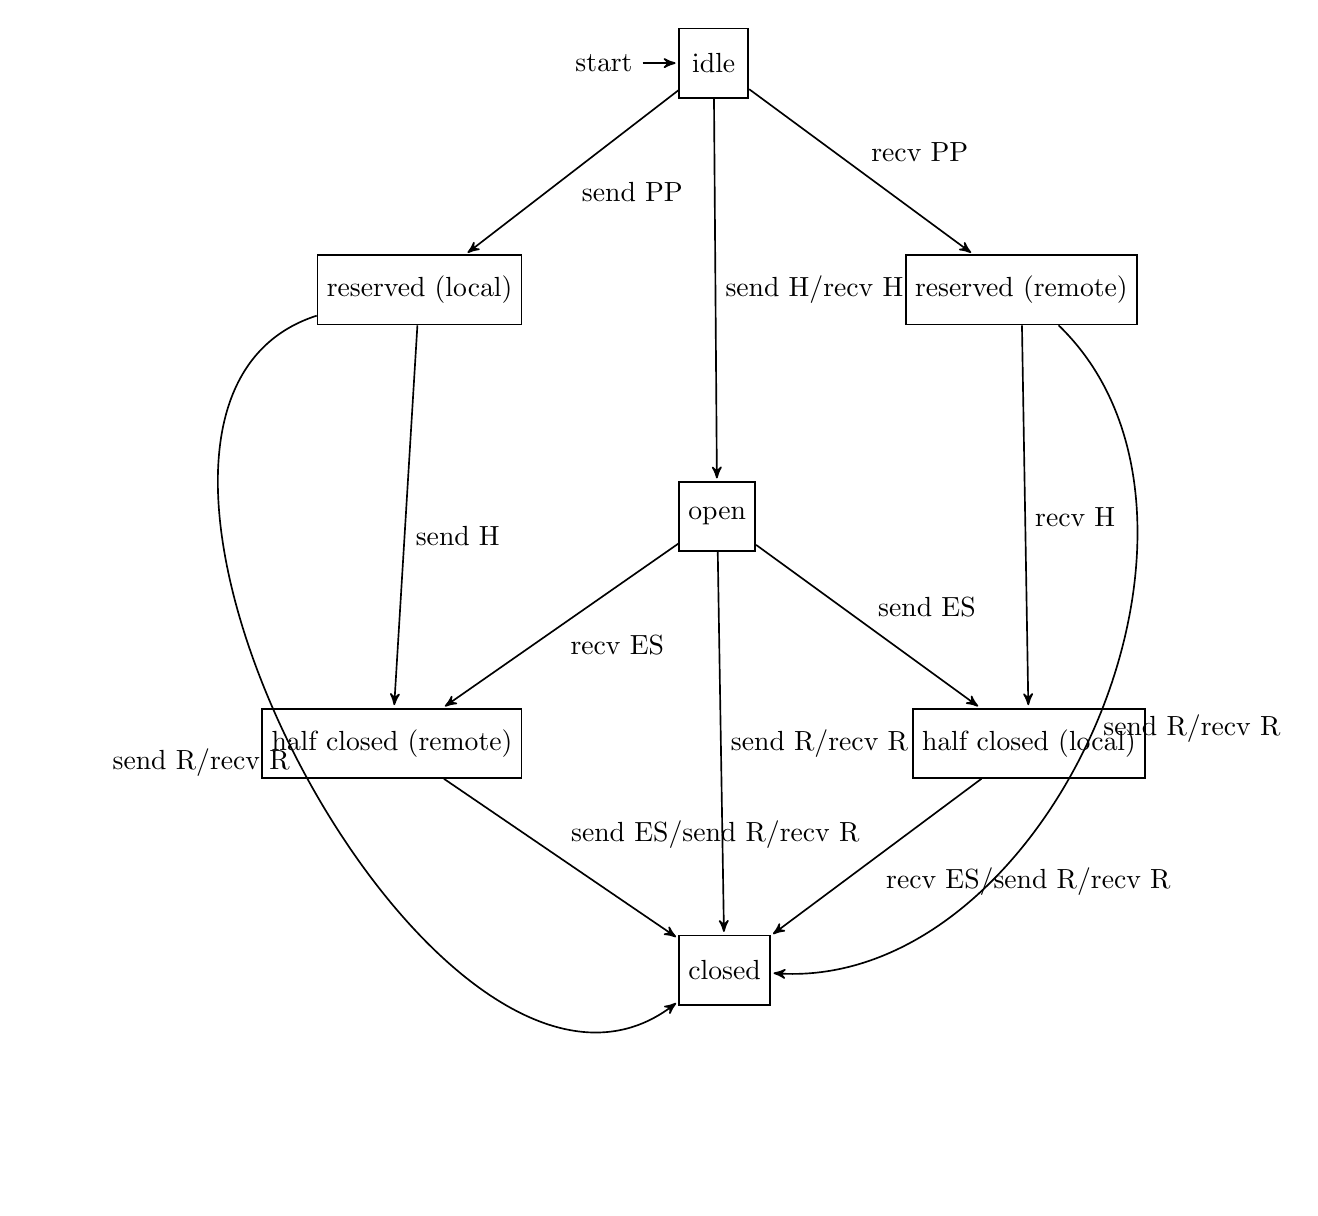
\begin{tikzpicture}[->,>=stealth',shorten >=1pt,auto,node distance=2.8cm,
	semithick]
	\tikzstyle{every state}=[draw, rectangle]

	\node[initial,state](idle){idle};

	\node[state, below left =of idle](rsv_loc){reserved (local)};
	\node[state, below right= of idle](rsv_rem){reserved (remote)};
	\node[state, below right =of rsv_loc](open){open};

	\node[state, below left=of open](hc_rem){half closed (remote)};
	\node[state, below right=of open](hc_loc){half closed (local)};

	\node[state, below right=of hc_rem](closed){closed};


	\path (idle) edge node {send PP} (rsv_loc)
	(idle) edge node {recv PP} (rsv_rem)
	(idle) edge node {send H/recv H} (open)
	(rsv_loc) edge [bend right=100] node[left] {send R/recv R} (closed)
	(rsv_rem) edge [bend left=70] node[right] {send R/recv R} (closed)
	(rsv_loc) edge node {send H} (hc_rem)
	(rsv_rem) edge node {recv H} (hc_loc)
	(open) edge node {recv ES} (hc_rem)
	(open) edge node {send R/recv R} (closed)
	(open) edge node {send ES} (hc_loc)
	(hc_rem) edge node {send ES/send R/recv R} (closed)
	(hc_loc) edge node {recv ES/send R/recv R} (closed)
	;

\end{tikzpicture}

http://http2.github.io/http2-spec/index.html\#StreamStates


\section{Measuring Web Performance}
\cite{han2015mwebmptcp}



\subsection{Categorizing web page components}

%Automatische Einstufung von Seitenbestandteilen (HTTP Requests) in Relevanz / User Utility
%-> nicht Thema der Arbeit, aber evtl. relevant f�r praktische Umsetzung

%Automatisches Aufbauen von Dependency Graphs


\section{Cooperation of Application Layer and Transport Layer}

% technical problems to be solved:
% *api needs to be defined
% *there might be a layer in between (Presentation Layer, TLS omnipresent today)

There are two main technical challenges in cooperation between (network) layers:

The first is that an adequate API needs to be defined. This is tricky especially in our case, the cooperation of application and transport layer, as one side is in user space and the other is a kernel component in modern operating systems.

The second challenge results from the fact that these layers are not directly adjacent to each other: In our case it is TLS encryption, which operates in the presentation layer, making all application layer data opaque to layers below. Therefore, a side channel needs to be established to allow information flow around the TLS encryption.
% see also: security considerations...


% research: what kinds of information that one layer has available, could provide an advantage to an other layer

research: what kinds of information that one layer has available, could provide an advantage to an other layer

\cite{Raisinghani_2004}
\cite{nowlan2012unorderedtcp}




%=====================================================================
\chapter{Approach}
%=====================================================================


\section{Optimizing the Multipath TCP Scheduler}

Several optimization approaches are considered in this chapter.

\subsection{Switching the scheduler based on content type or priority}
Many modern web pages consist of dozens of resources. They can be classified by their technical priority for rendering the page. 

1. The \textit{Document} is the main HTML file which is loaded first. It is strictly necessary for the browser to render the page, and to load subsequent resources. 

2. Synchronous Javascript resources (\texttt{<script>} tags) are required by the browser to construct the Document Object Model (DOM) tree. They must be loaded as soon as the tag is parsed by the browser.

3. Style sheets are needed for the first layout cycle of the page, which means usually nothing is displayed to the user until they are fully loaded.

4. Images can be loaded after the base frame of the site is visible, especially if the image size is provided in the Document source. The same is true for video, audio and most AJAX requests.

...

One can also look at their subjective utility to the user.

In the case of text heavy pages, like news sites, the Document and some images are most useful to the user as that contains the content of the page. In these cases, the Javascript resources are often providing tracking and advertising, so very important for the webmaster but annoying for the user. Especially tracking scripts can be delivered with lower priority as they are invisible and not time critical.

For interactive pages, the Javascript might provide all the relevant contents.   

...  ... 

Modern browsers and speed-optimized web pages make sure that the resources with the highest technical priority are requested first. The HTTP/2 server can also facilitate this by pushing out high-priority resources with HTTP Push.

The resources required for the first layout cycle will be handled by a scheduler with emphasis on low latency, like a redundant scheduler on lossy connections. The redundant scheduler sends all segments out on all paths to minimize delays caused by packet loss.

After these high priority resources are sent out, a regular, more bandwidth conserving scheduler can be used.



\subsection{Aggressive transmission of last segments}
The transmitting application signals the state of its outgoing buffers to the scheduler. An interesting condition occurs when the HTTP server has no more data to send, and only a few segments are left in the scheduler's queue. This means only these few segments are missing so that a complete web page can be rendered for the user. The scheduler can try to push out the missing segments more aggressively: By temporarily ignoring the available congestion window for the left over bytes, or by retransmitting on all available subflows.






\section{Choosing a web server platform}

To get information about the contents of the HTTP/2 application data, the cooperation of the web server is required.

\section{Security Considerations}
The information passed from the HTTP server to the MPTCP scheduler creates a side channel bypassing TLS encryption. It needs to be considered whether the passed data or the observable scheduler decisions based on this data could help an adversary. Some information are only protected by HTTP/2 and would be exposed on HTTP/1.1 connections anyway, like the length of individual resources. Others, like the content type, might be not available to the attacker otherwise.






%=====================================================================
\chapter{Implementation}
%=====================================================================


\begin{figure}[b]
	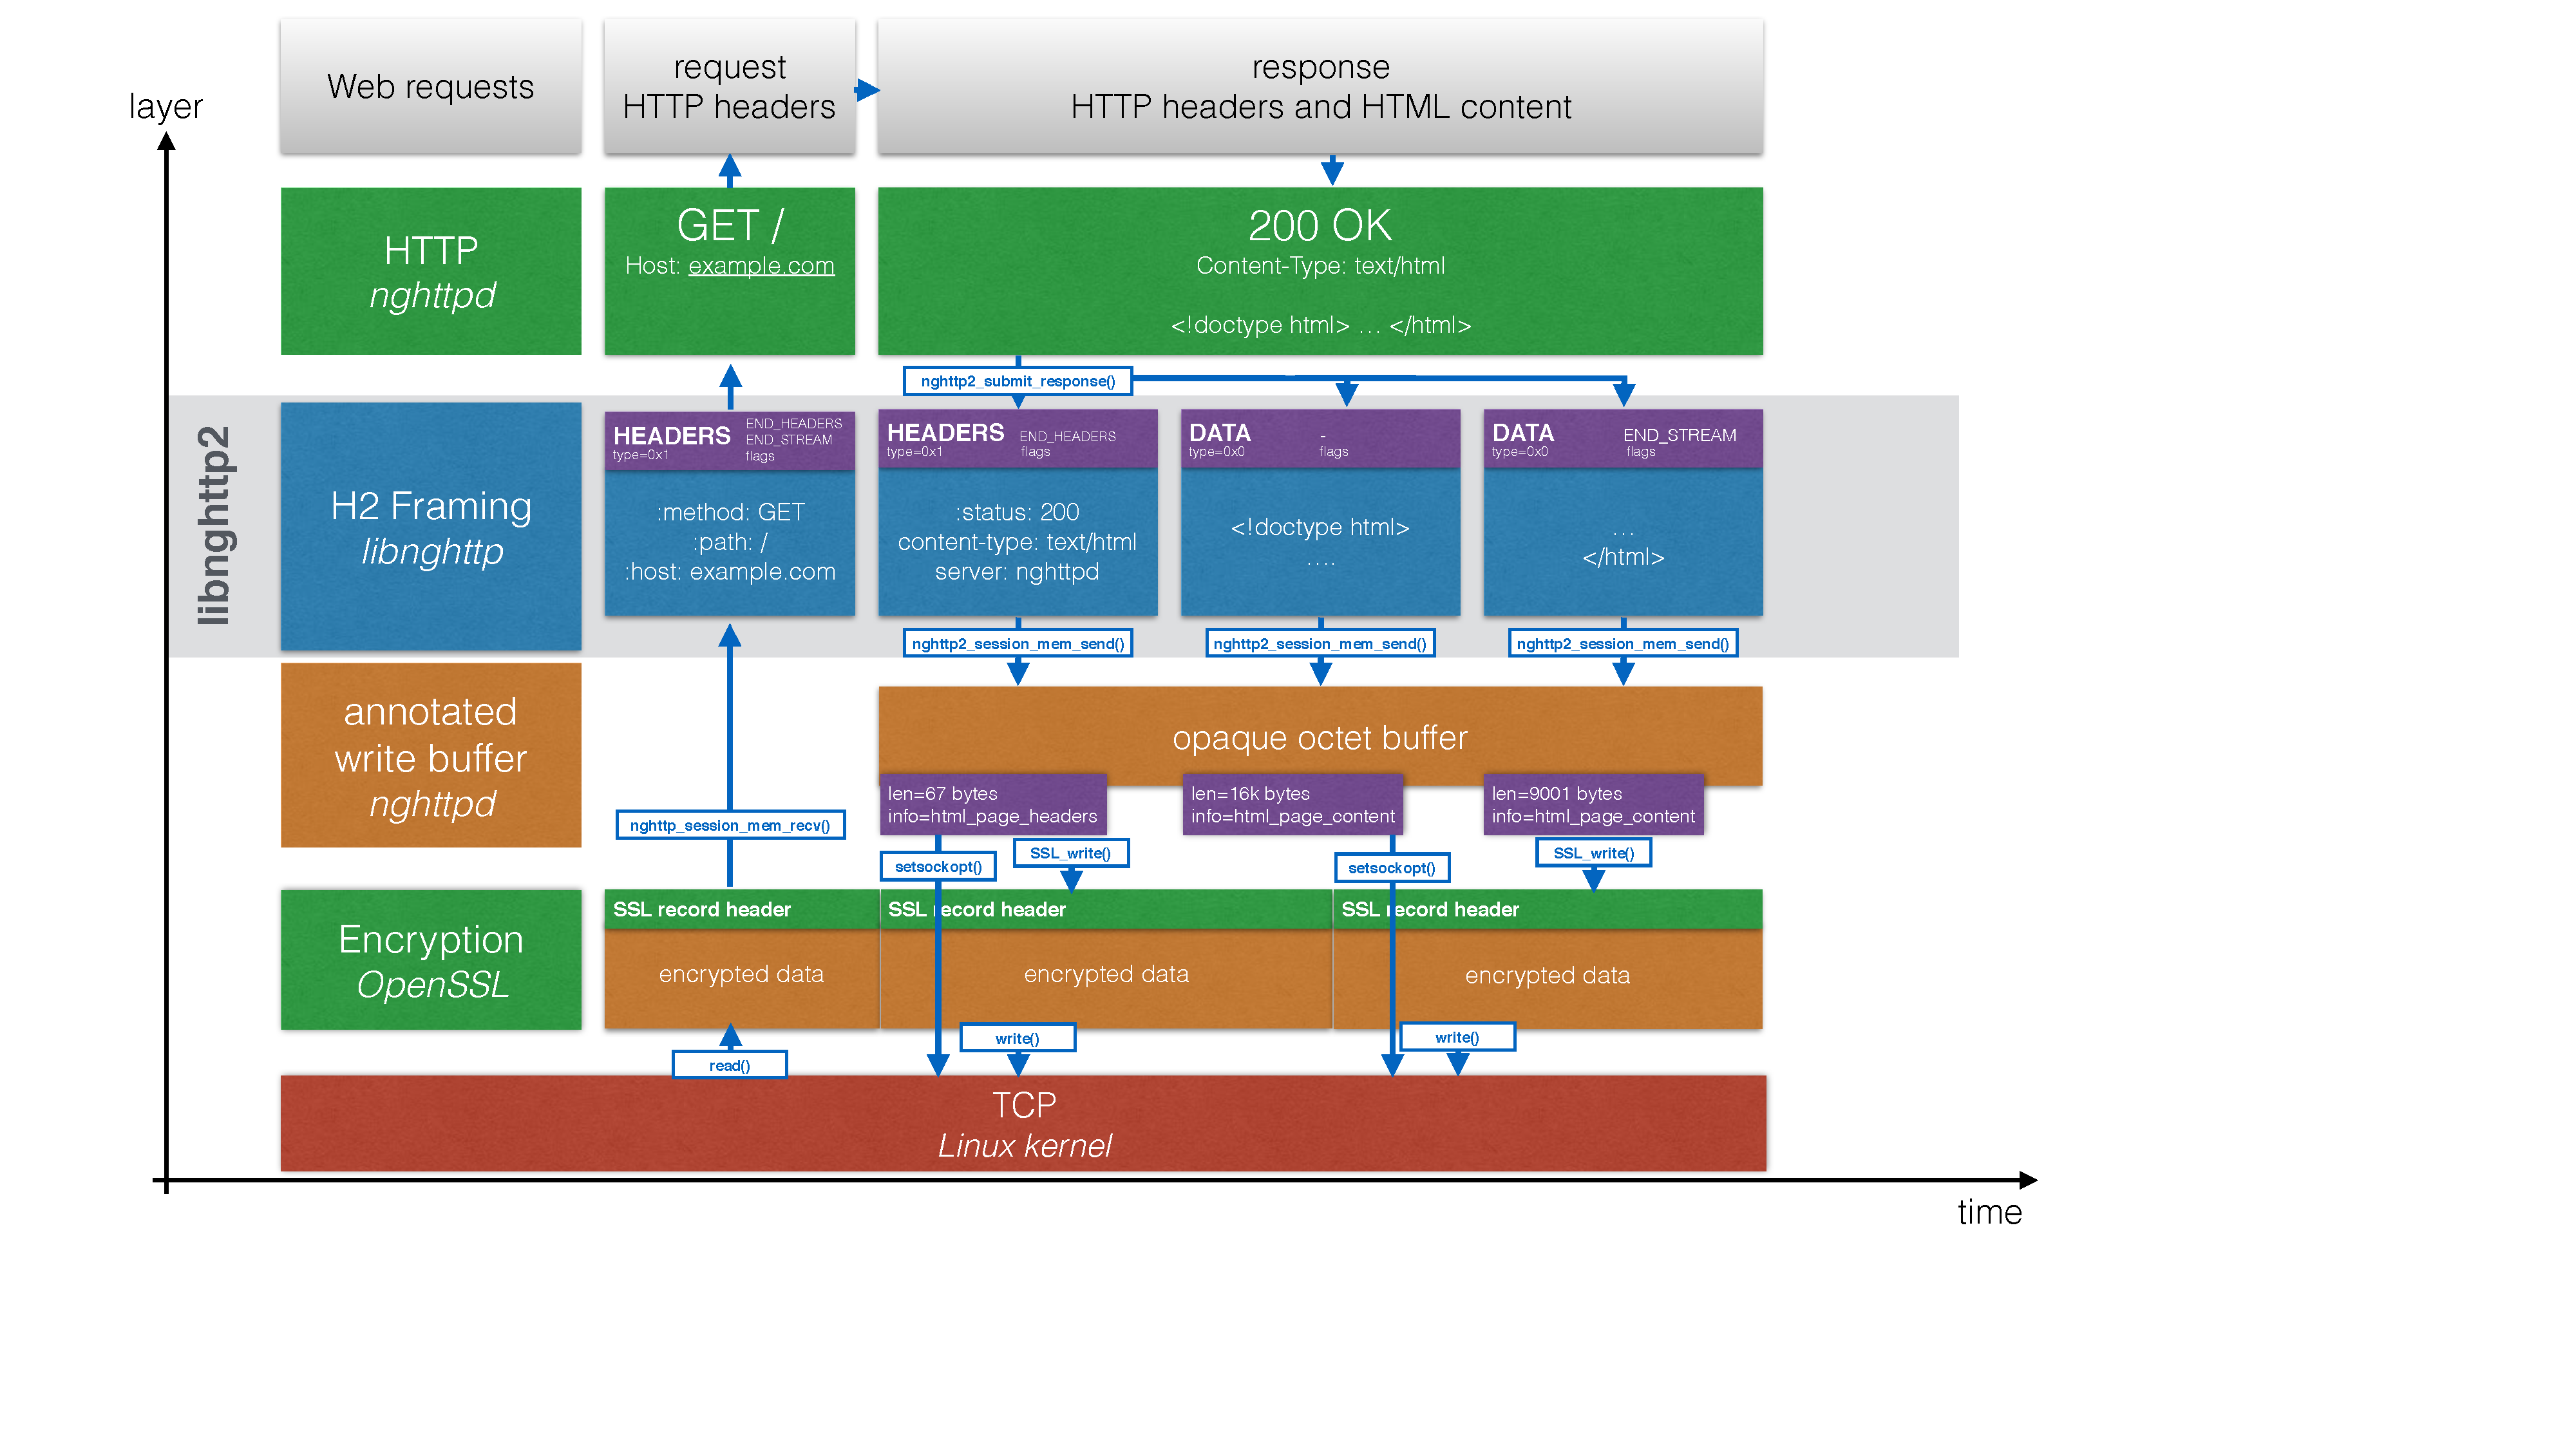
\includegraphics[width=1\textwidth]{http2-awb-layers.pdf}
	\caption{The annotated data's path through the application and network layer}
\end{figure}


\section{Transport Layer - Multipath TCP}

\subsection{TCP}


\subsection{Scheduler}


The scheduler algorithms are implemented in a scripting language. The scripts are just-in-time compiled and interpreted by the Rule Based Scheduler.



\subsection{Socket Buffers}



\section{Presentation Layer - OpenSSL}


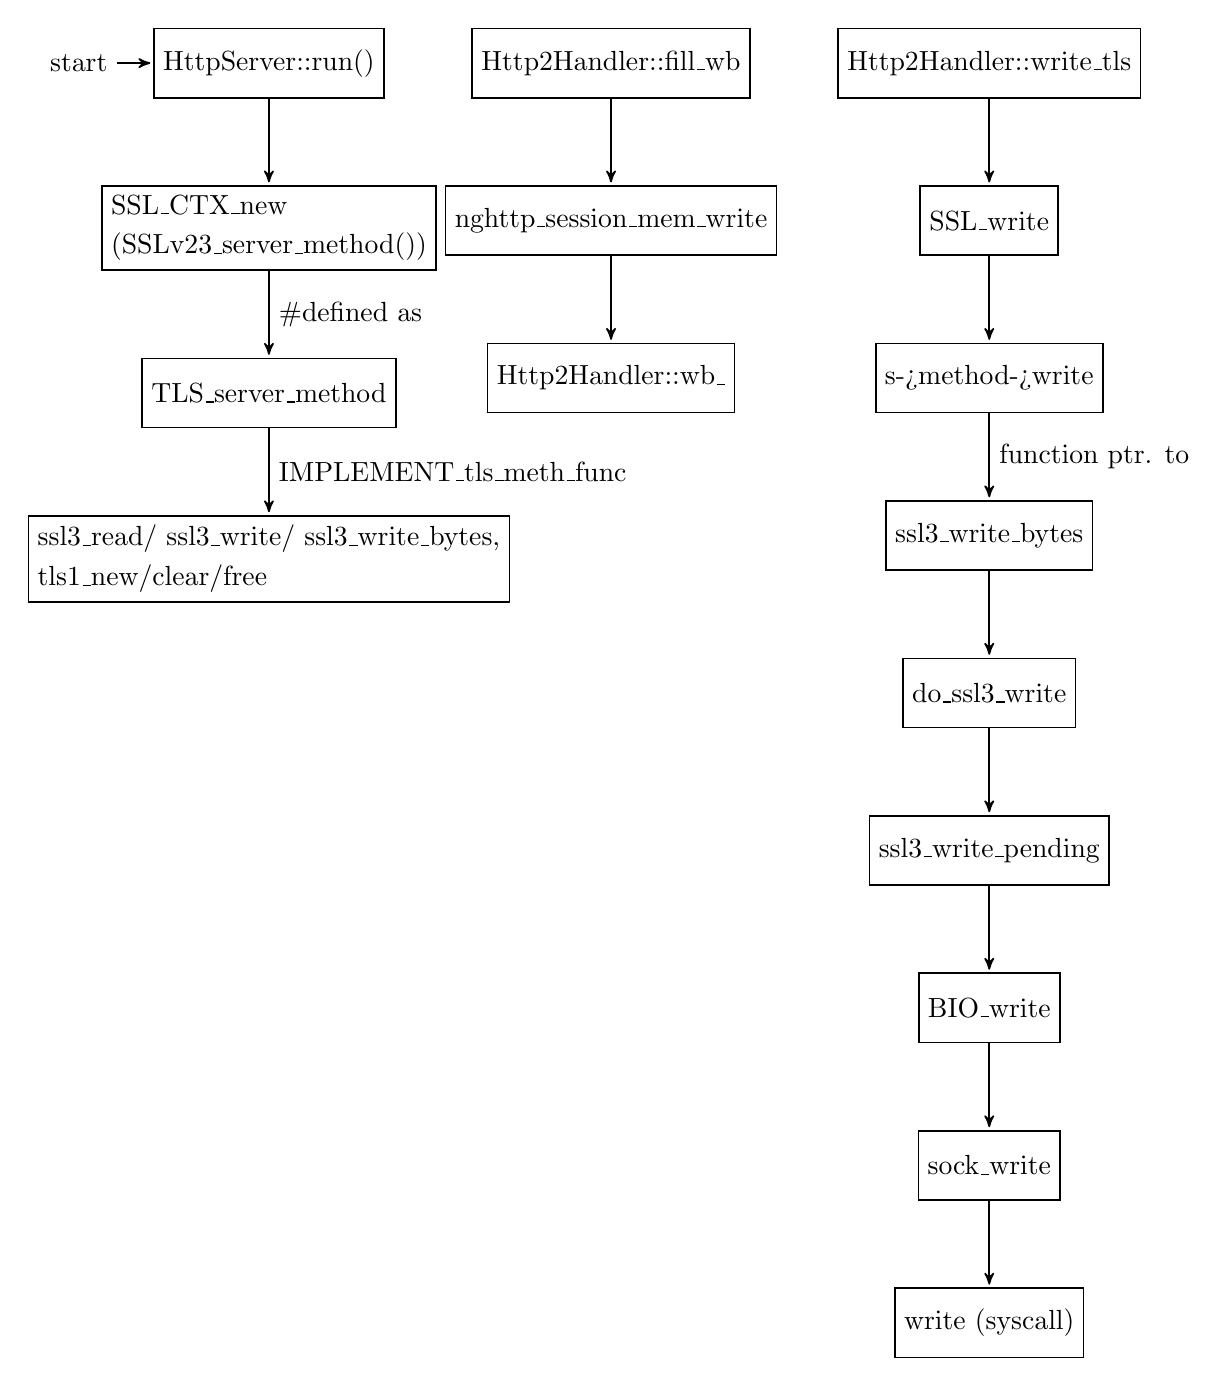
\begin{tikzpicture}[->,>=stealth',shorten >=1pt,auto,node distance=1.1cm,
		semithick]
	\tikzstyle{every state}=[draw, rectangle,
	execute at begin node={\begin{varwidth}{21em}},
	execute at end node={\end{varwidth}}]

	\node[initial,state](s1){HttpServer::run()};
	\node[state,below=of s1](s2){SSL\_CTX\_new \\(SSLv23\_server\_method())};
	\node[state,below=of s2](s3){ TLS\_server\_method  };
	\node[state,below=of s3](s4){ ssl3\_read/ ssl3\_write/ ssl3\_write\_bytes, tls1\_new/clear/free };


	\node[state,right=of s1](s6){  Http2Handler::fill\_wb };
	\node[state,below=of s6](s7){  nghttp\_session\_mem\_write };
	\node[state,below=of s7](s8){  Http2Handler::wb\_ };



	\node[state,right=of s6](s9){  Http2Handler::write\_tls };
	\node[state,below=of s9](sa){  SSL\_write };
	\node[state,below=of sa](sb){  s->method->write };
	\node[state,below=of sb](sc){  ssl3\_write\_bytes };
	\node[state,below=of sc](sd){  do\_ssl3\_write };
	\node[state,below=of sd](se){  ssl3\_write\_pending };
	\node[state,below=of se](sf){  BIO\_write };
	\node[state,below=of sf](sg){  sock\_write };
	\node[state,below=of sg](sh){  write (syscall) };

	\path (s1) edge (s2)
	(s2) edge node {\#defined as} (s3)
	(s3) edge node { IMPLEMENT\_ \\ tls\_meth\_func} (s4)

	(s6) edge (s7)
	(s7) edge (s8)

	(s9) edge (sa)
	(sa) edge (sb)
	(sb) edge node {function ptr. to} (sc)
	(sc) edge (sd)
	(sd) edge (se)
	(se) edge (sf)
	(sf) edge (sg)
	(sg) edge (sh)
	;


\end{tikzpicture}




\section{Application Layer - HTTP 2}






%=====================================================================
\chapter{Evaluation}
%=====================================================================



% overview of the chapter

% 1. decisions we made which have an impact on the evaluation:
%  -- using real web sites / hand-crafted sample web sites
%  -- if real web sites: which web sites to measure, how to prepare them for measurement
% - evaluation setup:
%  -- which browser to use for measurement
% - measured data points:
%  -- amount of data transmitted (overall, per interface/subflow)
%  -- complete page load time (onLoad)
%  -- load time of HTML Document
%  -- time to DOM Ready (doc + blocking scripts)
%  -- time to first render/paint
%  -- time to "`above the fold ready"' (this is probably the closest to user impression of load time)
%     - can be measured as the time of the last change above the fold
%  -- time to "`text ready"' (useful e.g. on newspaper sites where most users want to read the content only/first, but lot of slow crap is shown above the fold)

% 2. how the measurement is conducted (used browser, used additional scripts/extension to gather data from browser, additional scripts to gather transmitted data from network stack client/server side, automation, ...)
% -> this might also belong into Implementation???

% 3. results: data, graphs, observations, conclusions...



We have to decide which web sites to measure, and how to measure them.


\section{Selection of sample web pages}


- Self built test pages (plain html, small html file with many scripts/css, big html, etc ...)


Measuring the page load times of real-world web pages:

- Alexa Top Sites (or similar ranking)

- Hand-selected sites with interesting features / problems / optimization potentials

- Sites which are often used on mobile

\section{Preparation of real-world web sites}

% web sites need to be prepared
% some can be used as is
% on some, changes are inevitable, they won't work otherwise (https neccessary for h2, problems with third-party requests and dynamic content, etc)
% on some, we should change stuff, e.g. because there are optimizations for http/1.1 which make things worse on http/2 and it would be unrealistic to use them in this state
% etc.

\subsection{Handling dynamic and third party requests}

Downloading web pages with browser / wget and delivering with nghttpd - Problem: how to handle dynamic or third-party requests?

\begin{itemize}
	\item Cancel/reject all third party requests (in-browser / iptables)

	Pro: Easy, reproducible

	Con: not realistic (always a lot faster than real request)

	Pro: might be faster by the same amount, so still comparable (?)

	\item Let all third party requests through to the original sites

	Pro: Easy, realistic

	Con: dependent on network condition of test computer and load on original server (not reproducible)

\end{itemize}

Alternative: Use a caching HTTP/2 proxy (nghttpx, apache)

Pro: realistic (?), reproducible, (not that difficult either)

Con: ...


\section{How to measure page load speed }


\begin{wrapfigure}{r}{0.45\textwidth}
	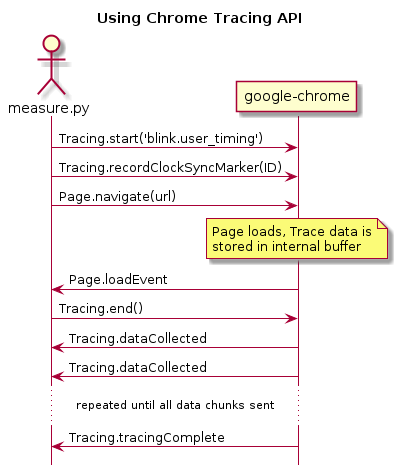
\includegraphics[width=0.4\textwidth]{chrome-tracing-api.png}
	\caption{A sample interaction with the Chrome Tracing API}
\end{wrapfigure}



\section{Measurements in simulated networks}

\subsection{Mininet}


\subsection{}


\section{Real world measurements}







%=====================================================================
\chapter{Conclusion}
%=====================================================================



\section{Outlook / Future Work}


% our work could be combined with :
Some optimizations rely on manually providing resource priorities and dependencies to the web server. Our work could be combined with automated algorithms to determine dependency graphs of web pages and user relevancy ratings of resources. Butkiewicz et al. \cite{klotski2015}

% - automated categorization of ressources/http requests

% - automated dependency graph

%Automatische Einstufung von Seitenbestandteilen (HTTP Requests) in Relevanz / User Utility
%-> nicht Thema der Arbeit, aber evtl. relevant f�r praktische Umsetzung

%Automatisches Aufbauen von Dependency Graphs



%=====================================================================
% Bibliography
%=====================================================================


\nocite{*}

\bibliography{thesis-h2-mptcp}{}
\bibliographystyle{plain}



\end{document}
